% !TeX root = ../main-paper.tex
\section{Dataset}
\label{sec:dataset}

% Conventions nommage
% Dataset annoté à la main = "ground truth"
% ground truth aligné = "ner-reference"
% entrées pero aligné = "ner-pero"
% entrées tesseract alignées = "ner-tesseract"




%In this work, we  aim  at  producing  structured  spatio-temporal  data  from the information contained in the XIX\textsuperscript{th} century Parisian trade directories.
%To do this, it is therefore necessary to extract the text from the scans of the directories to be processed and to identify the entries in the various indexing lists used.
%Then, in each of these entries, the named entities they contain have to be extracted to produce structured spatio-temporal data representing the evolution over time of the people and businesses listed in these directories, their descriptions and their locations.
%Both of these extraction tasks require data to train and evaluate the OCR and NER approaches identified as potentially relevant: Tesseract and PERO OCR for the OCR task and Spacy and CamemBERT - pre-trained or fine-tuned - neural models for the NER task.

This section presents the historical sources that we selected and their contents. It also details the construction of the groundtruth dataset leveraged in our experiments and the metrics used to evaluate OCR and NER results.

\subsection{A selection of Paris trade directories from 1798 to 1854}
\label{sec:corpus}

The directories are available from different libraries in Paris and have been digitised independently in various levels of quality. 
They cover a large period of time and originate from several publishers.
Therefore, their contents, indexes, layouts, methods of printing, etc. may vary a lot from one directory to another (see fig. \ref{fig:directories}).
We want our groundtruth dataset to be representative of the diversity of directories available in the period.

\begin{figure}[htb!]
	   \center{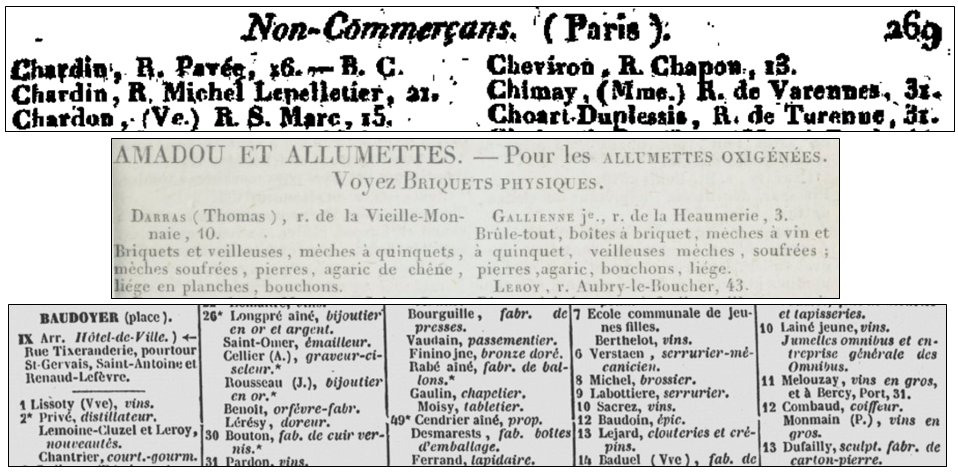
\includegraphics[width=0.9\textwidth]
	       {./images/DirectoryExcerpts2.png}}
	  \caption{\label{fig:directories} Examples of directory layouts and contents: 1) Duverneuil et La Tynna 1806 - index by name; 2) Deflandre 1828 - index by activity ; 3) Bottin 1851 - index by street name}
\end{figure}


Directories contain lists of people with various information attached.
For instance, the directory published by \emph{Didot} in 1854 contains three redundant lists of people sorted by name, by activity and by street name.
A typical example entry from this directory is ``\textit{Batton (D.-A.) \scalerel*{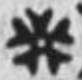
\includegraphics{./images/LH.png}}{H}, professeur au Conservatoire de musique et de déclamation, Saint-Georges, 47.}''.
It begins with the person's name and surname, here inside parentheses.
The glyph denotes that this person was awarded the \textit{Légion d'Honneur}.
Then comes a description of the person's activity, here his profession (professor at the Conservatory of music and declamation), but it can also be a social status.
Such descriptions range from a single word to paragraphs describing the occupation in full detail.
The street name and number where the person lives or carries out their activities ends the entry.

These are the pieces of information we want to extract, deduplicate and structure to build a spatio-temporal database.
Except for some potentially wordy activity descriptions, they correspond to named entities. However, while most entries contain the same types of named entities, their order and the way they are written vary from one directory/index to another. To provide examples of each entry structure, pages from each type have thus been annotated. %\footnote{In this work, the street name index entries have not been included as they are very different from the others. The strategy to be adopted to process them without loss of quality for the NER model will be the subject of future work.}.


\subsection{A dataset for OCR and NER evaluation}
\label{sec:dataset-for-eval}

\begin{figure}[tb]
    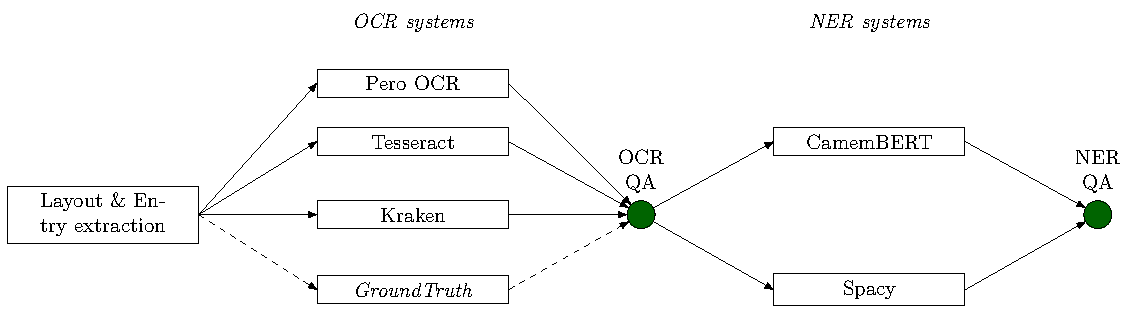
\includegraphics[width=\linewidth]{figs/protocol.pdf}
    \caption{Data extraction pipeline with two quality control checkpoints. The
    NER Q.A. checkpoint may either assess the NER system lonely (the dashed
    \emph{groundtruth} path) or may evaluate the joint work of a NER
    system with an OCR system.}
    \label{fig.pipeline}
\end{figure}


The simplified data extraction pipeline depicted in~\cref{fig.pipeline} processes the documents presented
in~\cref{sec:corpus}. First, the page layout extraction and entry segmentation are performed with a
semi-automated system and checked by a human. The resulting images, representing 8765 entries, are the inputs of a customizable two-stage pipeline.

%1. Entrée/Sortie de l'OCR
\textbf{OCR stage.} The first stage of the pipeline aims at extracting the raw text from the images. An OCR system runs
on the thumbnails of each segmented entry to extract its text. An entry might span over multiple text lines but is
always a single block. Thus, the most adapted mode is chosen when the OCR system allows for the detection mode (e.g. the
\emph{block} mode for \emph{Tesseract}). 
Some glyphs used in this dataset might be unknown to the OCR, and some like
\scalerel*{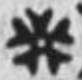
\includegraphics{./images/LH.png}}{H} do not even have a Unicode codepoint, and were annotated using Unicode Private User Area 1.
Furthermore, as some annotations guidelines where unclear to human annotators, some projections rules were applied: whitespace, dash, dots and a couple of commonly confused characters where projected to well-defined codepoints.
The same normalisation was applied to OCR predictions.
At the end of this first stage, an OCR Quality Assessment (Q.A.) between the \emph{normalised} groundtruth text and the
OCR output is performed on the basis of the $8,765$ entries which were manually controlled, totalling $424,764$ characters (including $54,387$ spacing characters). Entries are $49.0$-characters long on average.


%2. Entrée/Sortie
\textbf{NER Stage.} The second stage of the pipeline aims at extracting the named entities from a text with a NER
system. This text originates from the OCR outputs in a real-word scenario but might be the groundtruth text in order to
evaluate the NER performance independently. There are 5 types of entity to detect~(see.~\cref{tab.entities}).
The NER system has to classify non-overlapping parts of the text into one of these entities (or none of them). A second
Q.A. (namely, NER Q.A.) is performed at the end of this stage between the groundtruth and the NER output.

Note that the dataset used to assess the NER stage is a subset of the entries. Indeed, we need to ensure that the datasets
contain the same entries whichever the OCR used in the previous stage. Entries where the OCR produced an empty string
and those for which no entity could be projected from the groundtruth have to be ignored. 
We filter the set of entries by keeping only the entries that are always valid at the end of the stage 1.
%At the cost of losing 5\% of the references entries, we thus have 8341 valid entries at the input of the stage 2.
% /!\ True only for \peroocr and Tesseract predictions, not considering Kraken (we loose 500 more entries)
Therefore, the $8,765$ reference entries were manually annotated with $34,242$ entities; entries contain $3.9$ entities on average.
Projecting reference tagged entities on OCR predictions resulted in a variable loss of entries.
For \peroocr, $8,392$ valid entries were generated, for Tesseract $8,700$ and for Kraken $7,990$.
The resulting intersection of the sets of valid entries contained $7,725$ entries for the tree OCR systems (and the reference),
or $8,341$ entries if we consider \peroocr and Tesseract only.

\begin{table}
\caption{Entities to recognise in the dataset.}
\label{tab.entities}
\small
\begin{tabular}{llp{8cm}}
Entity & Count & Description\\    
PER & 8788 & a person name or a business name, usually referred to as several person names. First names, initials, or civility mentions are included. E.g.: \textit{Alibert (Prosper)}, \textit{Allamand frères et Hersent},\textit{Heurtemotte (Vve)}. \\
TITLE & 483 & an honorary title, either text, glyphs or a combination of the two. E.g: O. \scalerel*{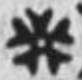
\includegraphics{./images/LH.png}} {H} for \textit{Officier de la Légion d'Honneur} or \scalerel*{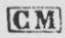
\includegraphics{./images/GMLondon.png}}{H} for the Great Medal at the London exhibition.\\
ACT & 6472 & the profession or social status of a person summarised in the single concept of activity. E.g.: \textit{horlogerie}, \textit{export en tous genres}, \textit{Conseiller d'État}, \textit{propriétaire}.\\
LOC & 9709 & mostly street names (\textit{r. de la Jussienne}), but may also be neighbourhoods (\textit{Marais du Temple}) or any indirect spatial references (\textit{au Palais Royal}).\\
CARDINAL & 8747 & a street number, as part of an address (16, 5 bis), or a range of numbers (e.g. 23-25 or 5 \textit{à} 9).\\
FT & 43 & a geographic entity type, used to give more details on a location, e.g. \textit{boutique}, \textit{atelier}, \textit{fab.} or \textit{dépôt}. \\
\end{tabular}
\end{table}


%
%TODO average number of tags/entities per entry
%TODO lists actual dataset content: set of entries. For each entry:
%\begin{itemize*}
%    \item ref to original book, page, region
%    \item human transcription (OCR GT)
%    \item human NER (NER GT)
%    \item [GENERATED] OCR produced by Pero OCR, Tesseract v4, Kraken (precise model used)
%    \item [GENERATED] NER GT aligned on text predictions from Pero OCR, Tesseract v4, Kraken
%\end{itemize*}


\subsection{Metrics for OCR and NER Quality Assessment}

\begin{figure}[tb]
    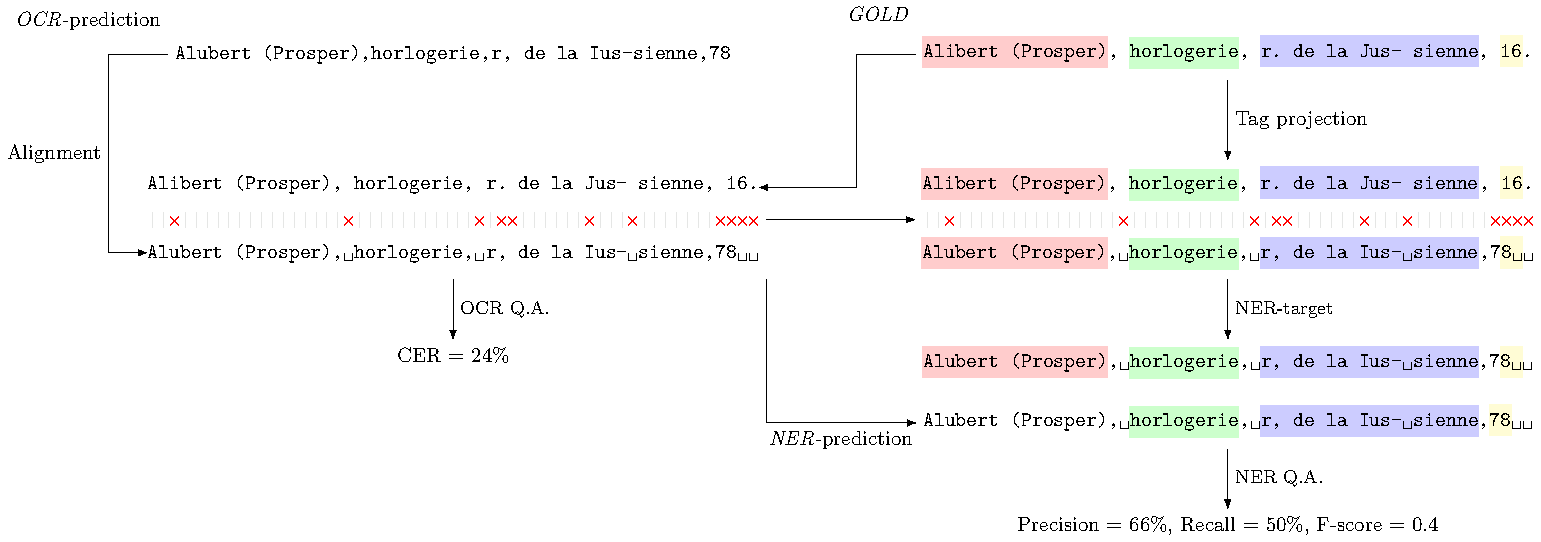
\includegraphics[width=\linewidth]{figs/eval-ocr-ner.pdf}
    \caption{OCR and NER evaluation protocol example.}
    \label{fig.eval-ocr-ner}
\end{figure}

\textbf{OCR Q.A.}  The predicted text by the OCR system is aligned with the groundtruth text using standard tools from
Stephen V. Rice's thesis~\cite{santos.2019.wcmel,neudecker.2021.whdip}. The Character Error Rate (CER) is computed at
the entry level and at the global level, defined as the ratio between the number of errors
(insertions/deletions/substitutions) over the reference text length.
Word Error Rate is hard to define for our tokens and was not considered.

%In this benchmark, we consider 3 OCR systems well known for historical document analysis: Pero OCR, Tesseract, and Kraken. 


\textbf{NER Q.A.}. The NER system outputs a text with tags that enclose the entities. To assess the quality of the
entity extraction, we rely on a technique similar as for the OCR evaluation to build the \emph{NER-target}. The
\emph{NER-target} is different from the groundtruth because it should not involve the errors committed during the
previous stages. The OCR text is first aligned with the groundtruth text to form the NER-\emph{input} (where
\emph{input} is a placeholder for \emph{pero} if the input text is from PERO, NER-\emph{tesseract},
NER-\emph{reference}\ldots). The tags of the groundtruth are then projected in the alignment on NER-\emph{input} to
provide the \emph{NER-target}. The NER system then runs on NER-\emph{input} and outputs the \emph{NER-prediction}. The
precision, recall, and f-measure (or f-score) are computed considering only the exact matches between entities of the
\emph{NER-target} and those from the \emph{NER-prediction}, i.e. pairs of entries for which the type, start and end positions are exactly the same.
Precision is the ratio of exact matches divided by the number of predicted entries,
and recall is defined as the ratio of exact matches divided by the number of expected entries;
the f-measure is their harmonic mean.

The evaluation process is illustrated on~\cref{fig.eval-ocr-ner}. The OCR and the groundtruth texts are first aligned to
evaluate the OCR accuracy. As there are 11 mismatches over 56 aligned characters, the CER is thus 24\%. This alignment
is then used to back-project the groundtruth tags to build the tagged NER-\emph{target}. Finally, the NER system runs on the
OCR text; its output is compared to the NER groundtruth. There is only 2 over 3 tags matching in the prediction (precision),
while only 2 over 4 entities are matched in the reference (recall). It follows an overall f-score of 0.4.
%
% A side effect of tag projection is that it can produce degenerated tags, i.e. empty or containing only spaces.
% In such cases, the corresponding entries must be removed from the dataset,
% and only the intersection of the sets of valid entries must be used to compare NER systems with multiple OCR predictions or references.
